\documentclass[fleqn,10pt]{wlpeerj}
\title{Assembly on Cloud 9: Assembly metric assessment using Transcriptomes of closely related Ascidian species}

\author[1]{Elijah K. Lowe}
\author[2]{Billie J. Swalla}
\author[3]{C. Titus Brown}
\affil[1]{Michigan State University, Computer Science and Quantitative Biology, East Lansing, Michigan, 48823, USA}
\affil[2]{University of Washington, Biology Department and Friday Harbor Laboratories, Seattle, Washington, 98195, USA}
\affil[3]{Michigan State University, Computer Science and Microbiology and Molecular Genetics, East Lansing, Michigan, 48823, USA}

\keywords{Assembly, Cloud computing, Ascidians, Next-gen sequencing}

\begin{abstract}
\textit{De novo} transcriptome sequencing and assembly for non-model organisms has become prevalent in the past decade. However, most assembly approaches are computationally expensive, and little in-depth evaluation has been done to compare \textit{de novo} approaches. We sequenced several developmental stages of two free-spawning marine species\textemdash\textit{de novo} and \textit{Molgula oculata}\textemdash and assembled their transcriptomes using four different combinations of preprocessing and assembly approaches, and evaluated the quality of the assembly. We present a straightforward and reproducible mRNAseq assembly protocol that combines quality filtering, digital normalization, and assembly, together with several metrics to evaluate our \textit{de novo} assemblies. The use of digital normalization in the protocol reduces the time and memory needed to complete the assembly and makes this pipeline available to labs without large computing infrastructure. Despite varying widely in basic assembly statistics, all of the assembled transcriptomes evaluate well in metrics such as gene recovery and estimated completeness.
\end{abstract}

\begin{document}

\flushbottom
\maketitle
\thispagestyle{empty}

\section{Introduction}

Next generation sequencing (NGS) has allowed us to study organisms with a broader lens, looking at entire genomes and transcriptomes instead of single genes.  This capability is particularly important for non-model organisms where little prior knowledge may be available, and where NGS readily enables whole-transcriptome analyses \citep{wang_rna-seq:_2009}, allowing comparisons in organisms that are ecologically or evolutionarily interesting, amongst other biological applications.

There are now several sequencing technologies, Illumina being one of the most versatile \citep{glenn_field_2011}, that can produce millions of short reads ranging from 75 to 150 bp in length at a low cost \citep{zhang_impact_2011}. As sequencing costs continue to drop, transcriptomes from multiple developmental stages of non-model organisms can easily be sequenced. Various types of \textit{de novo} assembly algorithms and reference based assembly approaches have been developed to handle this massive influx of transcriptomic data \citep{pop_genome_2009,vinson_assembly_2005,stapley_adaptation_2010}. It has been shown in some cases that mapping mRNA-seq reads to a reference genome yields better transcriptomes than \textit{de novo} assemblies, even if the genome is 5-15\% divergent \citep{vijay_challenges_2012}. However, with many non-model organisms, no nearby reference genome is available.

\textit{De novo} transcriptome assembly is the only solution for organisms with no evolutionarily close reference genome.  Transcriptome assemblers such as Trinity \citep{grabherr_full-length_2011} and Velvet/Oases \citep{zerbino_velvet:_2008,schulz_oases:_2012}, use De Bruijn-graph based \textit{de novo} approach which build graphs connecting the reads based on k-mer connectivity,  and are then traversed via an Eulerian path algorithm to assemble transcripts. Because De Bruijn graphs are based on exact matches between DNA words, increasing numbers of sequencing errors result in an exponential number of new paths, adding to the complexity of the graph and, in turn, increasing the assembly time and memory requirements \citep{pop_genome_2009}.

Here we have sequenced the transcriptomes of several developmental stages of \textit{Molgula occult} and \textit{Molgula oculata}\textemdash two closely related, free-spawning ascidian species, with no available reference genome. \textit{Ciona intestinalis} and \textit{Ciona savignyi} are the closest related ascidian species with well-assembled genomes, but are not close enough to use as a nucleotide reference for transcriptome construction. In this paper, we describe an efficient, easy to follow protocol for the transcriptome assembly of two Molgulid developmental transcriptomes. A crucial part of this protocol is the use of a preprocessing step that normalizes read abundances prior to assembly, called ``digital normalization.'' We study the effect of digital normalization on assemblies performed with both Trinity and Velvet/Oases.  We compare our approach to the results of running Trinity and Velvet/Oases without digitally normalized reads and show that our approach recovers essentially the same gene content but has significantly reduced requirements for time and memory.  This reduction in time and memory lets us assemble transcriptomes efficiently using cloud resources, making our results exceptionally easy to reproduce \citep{haas_novo_2013}, and more broadly enabling transcriptome assembly by researchers without access to large computer resources.

\section{Methods}
\subsection{Sequencing preparation}
\textit{M. occulta} and \textit{M. oculata} were collected by dredging off the shores of Roscoff, France near La Station Biologique. Swalla et al have previously described the maintenance \citep{swalla_interspecific_1990} and culturing \citep{swalla_multigene_1999} of the animals. The transcriptomes of \textit{M. occulta} and \textit{M. oculata} were sequenced at Michigan State University (MSU) in the Research Technology Support Facility on Illumina HiSeq 2000. Five lanes of sequences were generated for \textit{M. occulta}, two lanes of the gastrula stage (F+3), one of neurula (F+4), one of early tailbud (F+5), and one from the tailbud (F+6) stage (Table 1). Three lanes of sequences were generated for \textit{M. oculata}, one each for the gastrula, neurula and tailbud stage. 10$\mu$g of RNA were sequenced for each stage with the exception of \textit{M. occulta} F+4, where 1.05$\mu$g of RNA was sequenced. On average each embryonic stage yielded 48 million reads of 75 base pairs (bp) in length with paired-end insert lengths of 250 bp. All reads can be found in the NCBI short read archive (SRA) under accession number SRP040134. 

\subsection{Assembly protocol}
Below is an overview of the steps used for the \textit{de novo} assembly and annotation of our transcriptomes.
\begin{enumerate}[noitemsep] 
\item Quality trimming and filtering of raw reads.
\item Apply digital normalization to decrease data size.
\item Assemble transcriptome.
\item Assess transcriptome quality.
\item BLAST (gene recovery/identification).
\end{enumerate}
Scripts used to run these steps can be found in the following github repository: https://github.com/ged-lab/2014-mrnaseq-cloud
\subsection{Pre-assembly read trimming and normalization} 
Low quality bases were trimmed and low quality reads were removed using quality-trim-pe.py found in the scripts directory of the repository. A hard trim is done at a Phred quality score of 33 and reads less than 30 base pairs are discarded. This process creates a paired and singleton fastq file for each library because of the removal of low quality reads. The filtering of reads allows for better assembly and better mapping, although it may also reduce sensitivity to low-expressed transcripts \citep{lohse_robina:_2012, macmanes_optimal_2014}. The reads were initially 75 bp long, and the average base pair (bp) length was 63 bp after quality trimming and filtering. After quality trimming reads were either directly assembled, or first preprocessed with digital normalization and then assembled. 

Digital normalization (diginorm) is a technique that down samples reads from highly abundant transcripts while retaining approximately the full sequence information content of the reads \citep{brown_reference-free_2012}. Here, for each species, reads from all stages were normalized together to build a common reference transcriptome; reads were normalized to a k-mer coverage of 20 with the k-mer size set to 20 as well.  The initial data set from \textit{M. occulta} contained 237 million reads from 5 lanes, and \textit{M. oculata} contained 150 million total reads; after digital normalization, the \textit{M. occulta} dataset was reduced to 91.6 million reads and \textit{M. oculata} was reduced to 50 million reads, a ~60\% and ~77\% reduction respectively (Table~\ref{fig:time_and_memory.pdf}).

\begin{table}[ht]
\centering
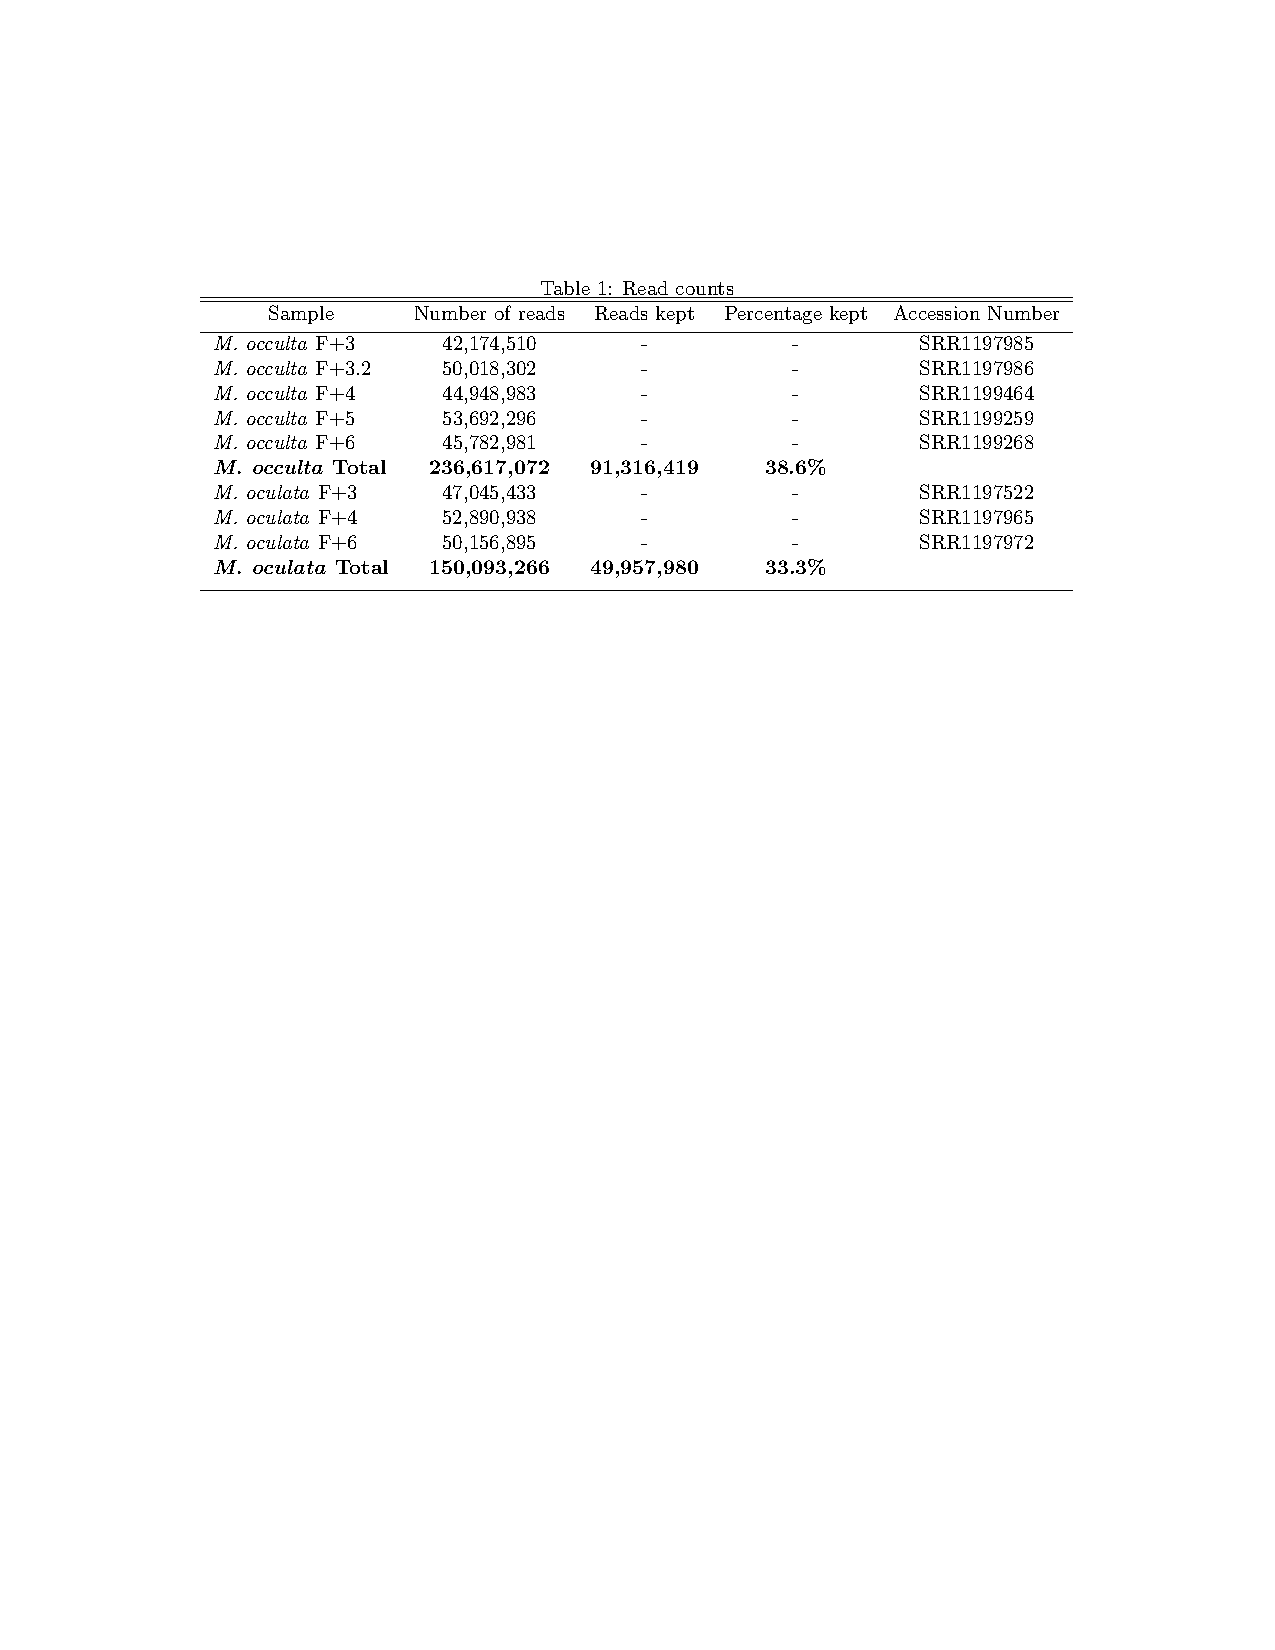
\includegraphics[scale=1.0]{Table1.pdf}
\caption{\textbf{Digital normalized reads.} The number of reads sequenced before and after digital normalization are shown for each lane of sequencing. The percentage of total reads kept after digital normalization is shown in bold. \textit{M. occulta} had approximately \mytilde237 million reads and was reduced to 91 million reads, a 60\% reduction. \textit{M. oculata} had 150 million reads and reduced by 77\% to \mytilde50 million reads. }
\label{fig:Table1.pdf}
\end{table}

\subsection{Transcriptome assembly}
We used the Trinity (r20140413p1) and Velvet/Oases (v1.2.08/v0.2.08) assembler packages, both of which have performed well on other data sets \citep{vijay_challenges_2012,grabherr_full-length_2011,schulz_oases:_2012}.  Velvet was initially developed to assemble genomes, and the Oases add-on package was developed for transcriptome assembly, since transcriptomes have variable coverage and many isoforms.  Since Oases cannot be run without Velvet, we refer below to transcriptomes assembled with Velvet and Oases as Oases assemblies. Unlike Trinity, Oases requires the choice of a k-mer overlap for assembly; we chose several k values ranging from k = 21 to k = 35, for odd values of k, with scaffolding turned off. After assembly, the Oases transcriptomes with the highest number of blast hits to \textit{C. intestinalis} were selected for further analysis. The Trinity assembler was run with default parameters.

All assemblies were performed on the Michigan State University (MSU) High Performance computing cluster (HPCC).  All diginorm assemblies were repeated on Amazon EC2 machines as a proof of concept.
After assembly, transcripts shorter than 200 bp in length were removed, and CD-HIT was used to eliminate small transcripts with 99\% identity to longer transcripts using the following command: ``cd-hit-est -i \textless transcript file\textgreater -c 0.99 -o \textless output file\textgreater'' \citep{li_cd-hit:_2006}.

To choose the best k-mer parameter for the Oases assemblies, \textit{C. intestinalis} proteins were searched with TBLASTN (e-value cutoff of 1e-6) against each Oases assembly and the transcriptome with the most hits was selected for further analysis.
\subsection{Gene identification}
We used standalone BLAST to find reciprocal best hits (RBH) between the eight assembled transcriptomes and the \textit{C. intestinalis} proteome from the NCBI under search term ``(ciona intestinalis) AND Ciona intestinalis [porgn:\_\_txid7719]''. At the time of retrieval there were 16,123 sequences and they were downloaded and stored in the github repository under the file name ``ciona\_transcriptome.fa'' in case the sequences change on the NCBI. An e-value cutoff of 1e-6 was used as a minimum threshold for transcript identity.  The find-reciprocal-2.py script was used to identify the RBH.
\subsection{Read mapping}
	To determine the inclusion of reads in the various transcriptome assemblies trimmed reads were mapped to their respective species using bowtie2 v2.2.1 \citep{langmead_fast_2012}. For both unnormalized read and diginorm assemblies the full set of trimmed reads were used for mapping. Default parameters were used, and both paired ends and singletons were mapped. Samtools v0.1.19 \citep{li_sequence_2009} was used for format conversion from SAM to BAM format, and also to calculate the percentage of mapped reads. The BAM files were also used to calculate the coverage of transcripts.

\section{Results}

\subsection{Digital normalization reduces the resources needed for assembly}
 The \textit{M. oculata} unnormalized read data set assembled with Oases used 44 CPU hours and 85 GB of RAM. The Oases assembly done with the digitally normalized reads took \mytilde22 CPU hours and 21 GB of RAM (Figure~\ref{fig:time_and_memory.pdf}); this includes the time and memory required to run the digital normalization pipeline. \textit{M. occulta} diginorm Oases assembly required over 100 GB of RAM, and the raw read Oases used 300 GB of RAM. The raw read Oases assemblies for both species took twice as long and needed at least three times as much memory when compared to the diginorm reads.

The difference in assembly time and memory between diginorm and raw reads was not as large when using the Trinity assembler. Diginorm completed its assemblies several hours faster than assembling raw reads, \mytilde15 hours compare to \mytilde26 hours for \textit{M. oculata} and \mytilde24 hours compared to \mytilde39 hours for \textit{M. occulta}. \textit{M. occulta} assembled with 23.17 GB of RAM for assembling the normalized reads versus 34.14 GB of RAM for the unnormalized reads (Figure~\ref{fig:time_and_memory.pdf}).

\begin{figure}[tbp]
\centering
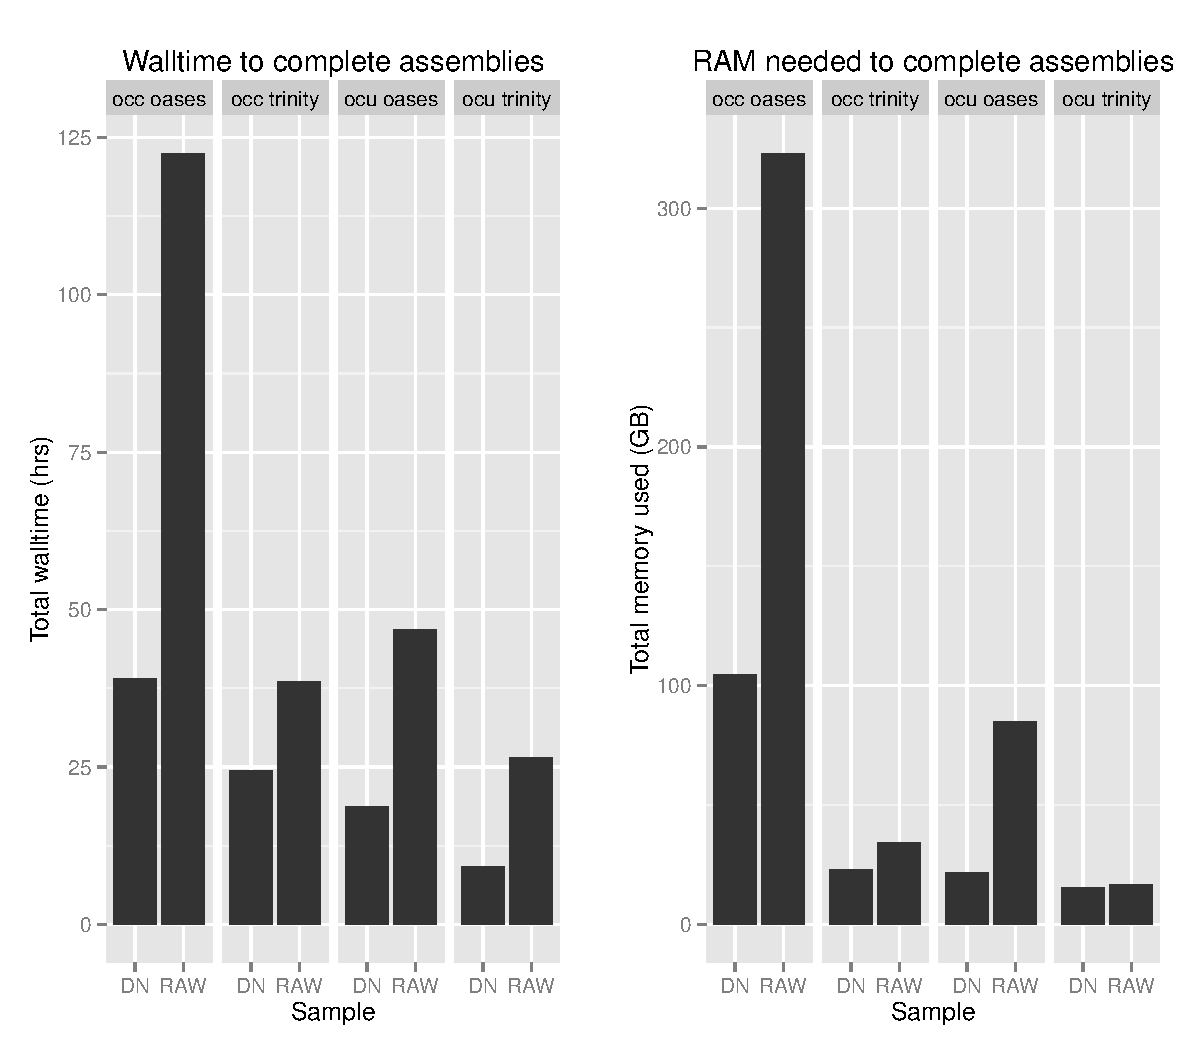
\includegraphics[scale=0.5]{figure_1_time_and_memory.pdf}
\caption{\textbf{Wall time and memory requirements for assemblies.} Wall time (left) in hours to complete the diginorm (DN) and raw read (RAW) assemblies for both species and assemblers. Oases assembled multiple k's, 21 $\leq$ k $\leq$ 35 opposed to Trinity that assembles a single k. This is one reasons the assembly times differed. (right) Shows the memory used to assemble each of the transcriptomes. M. oculata (ocu) transcriptomes assemble in less time than M. occulta (occ) because they have less lanes of reads to assemble. In all cases diginorm required less time and memory to complete the assembly.}
\label{fig:time_and_memory.pdf}
\end{figure}
  
\subsection{Assembly statistics varied by preprocessing approach and assembler}
Oases run with the diginormed reads yielded fewer total transcripts than Oases run with the unnormalized reads. The \textit{M. oculata} diginorm assembly produced 300 fewer transcripts, and the \textit{M. occulta} diginorm assembly produced 227 less transcripts (Table~\ref{fig:Table2.pdf}). Digital normalization had the opposite affect when using Trinity for assembly, increasing the total number of assembled transcripts by 7,840 for \textit{M. oculata} and 9,197 for \textit{M. occulta}.

\begin{table}[tbp]
\centering
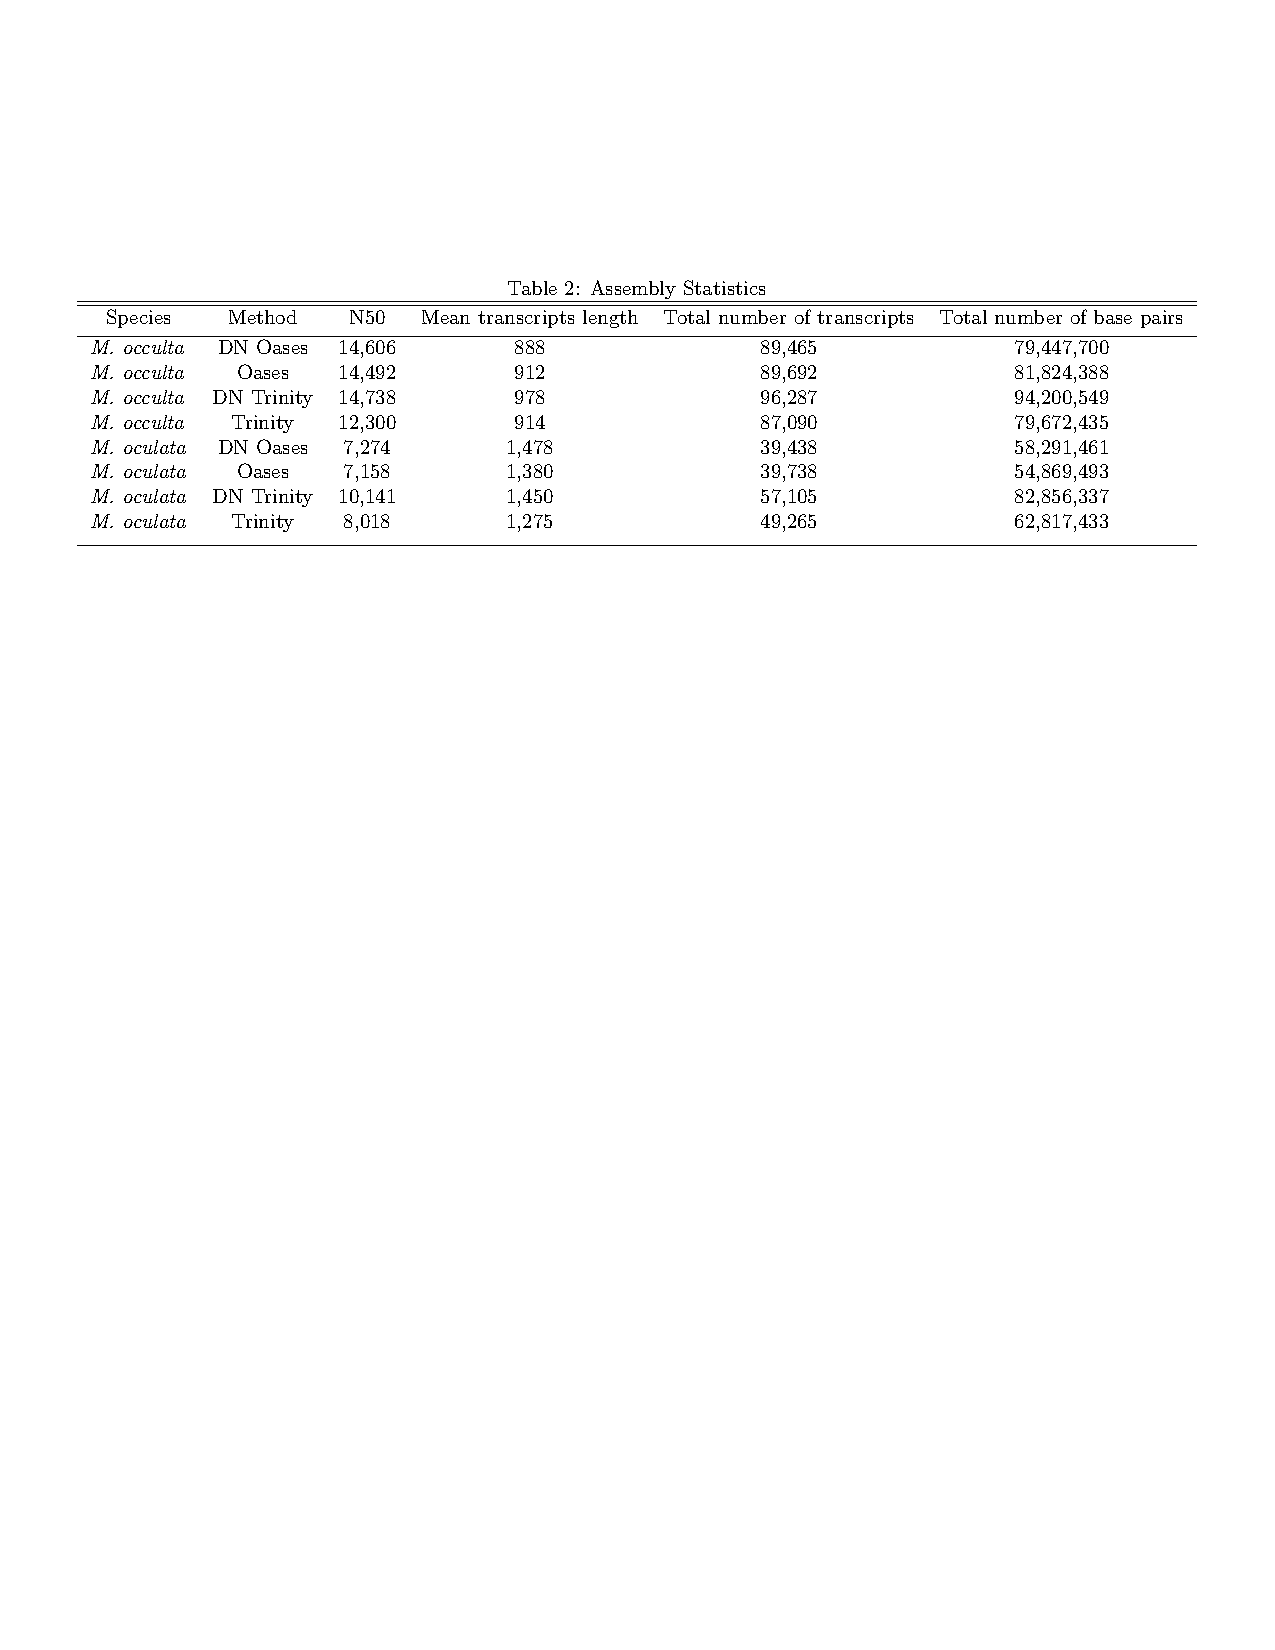
\includegraphics[width=\linewidth]{Table2.pdf}
\caption{\textbf{Transcriptome metrics.} Several metrics used to assess the quality of the assembled transcriptomes. The N50, mean transcript length, total number of transcripts and total number of base pairs are listed for each transcriptomes. These are typically the metrics used to assess the quality of a transcriptome. Although some of these metrics such as N50 are suitable for genomes, they are not as useful for transcriptomes}.
\label{fig:Table2.pdf}
\end{table}
   
Trinity produces 6.8k (7.6\%) more transcripts than Oases for \textit{M. occulta} using the digitally normalized reads, and a 2.6k (2.9\%) decrease in the number of transcripts using the unnormalized reads. Trinity assembled more transcripts for both \textit{M. oculata} assemblies, a 17.6k (44.8\%) increase for diginorm and a 9.5k (24\%) increase for the raw reads. 

\subsection{Trinity assemblies include more low-abundance k-mers than Oases assemblies}
We next examined the k-mer spectrum of the assembled transcripts using k-mer abundances from the digitally normalized reads. The k-mer spectrum is an account of the information content of the reads and can be used to evaluate the ability of the assemblers to recover low-abundance transcripts \citep{pop_genome_2009}.  We first used digital normalization to reduce the reads to a median k-mer coverage of 20, so that the k-mer frequency spectrum peaked at a coverage of 20, and then plotted a cumulative abundance plot of those k-mers shared between the normalized reads and the assemblies. The results, displayed in Figure 2, show that Trinity recovers more low-abundance k-mers.  Also note that between assemblies done with the same assemblers, the k-mer distributions were very similar, suggesting that the k-mer spectrum is reflective of the underlying graph traversal algorithm used by the assembler. In addition the Trinity assemblies included more unique kmers (Figure~\ref{fig:multiplicity})

\begin{figure}[tbp]
	\begin{center}
	\subfigure[]{%
                \label{fig:figure_2_Mocc_dist}
                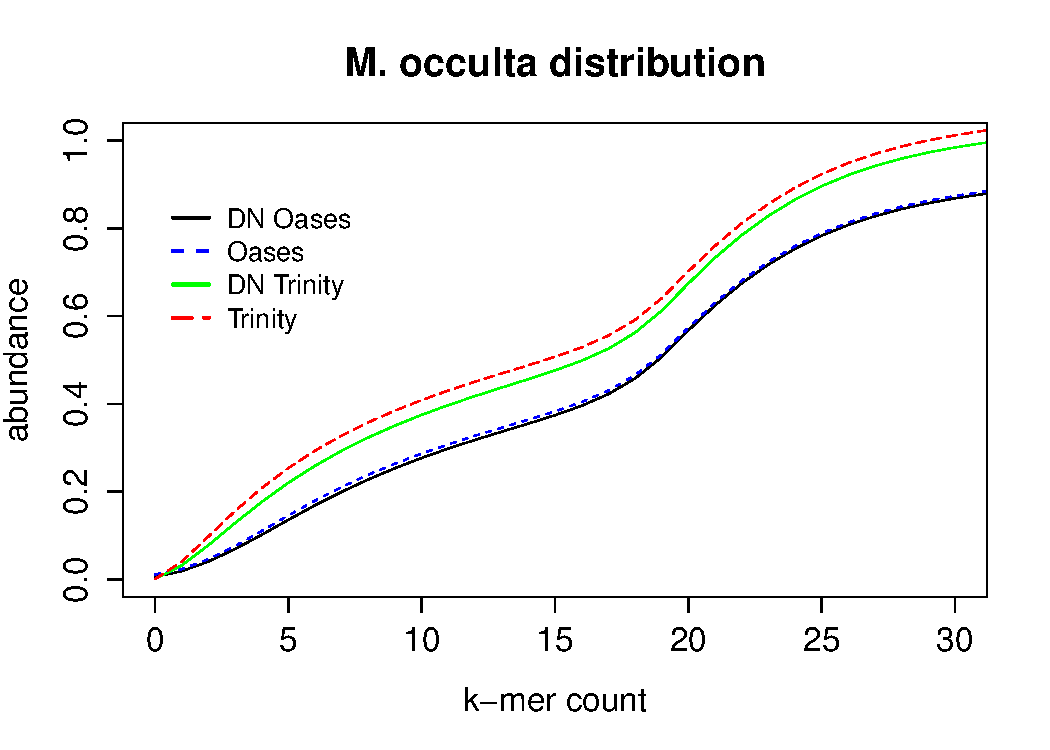
\includegraphics[width=0.4\textwidth]{figure_2_Mocc_dist.pdf}
	}%
	\subfigure[]{%
                \label{fig:figure_2_Mocu_dist}
                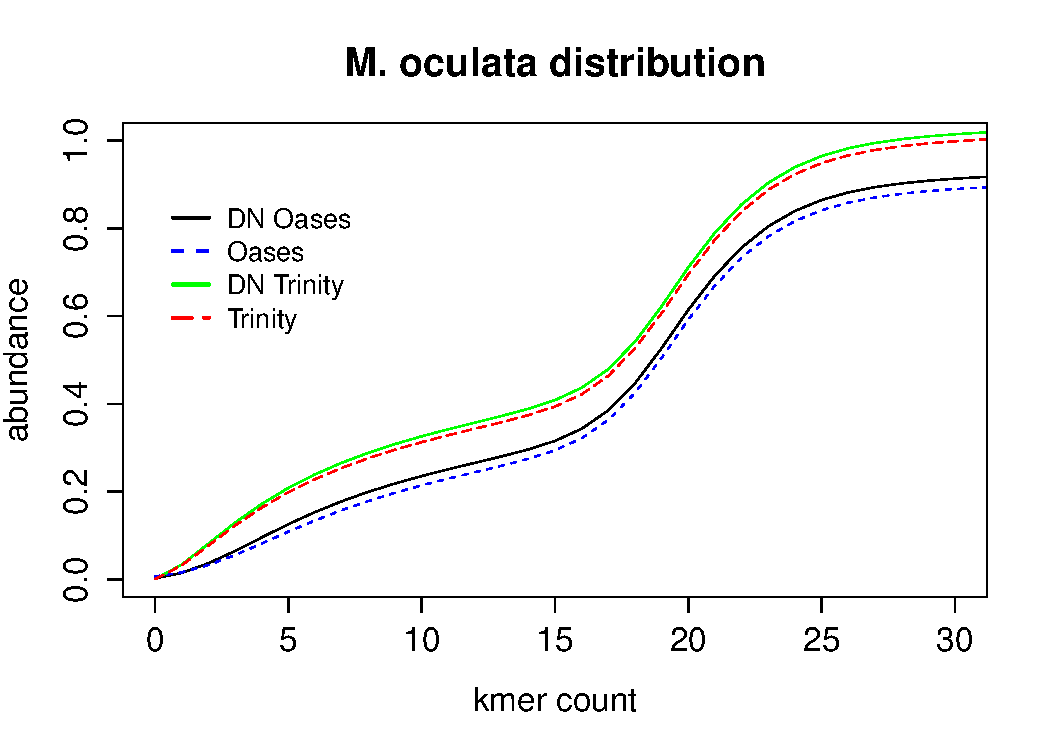
\includegraphics[width=0.4\textwidth]{figure_2_Mocu_dist.pdf}
	}%
	\end{center}
	\caption{\textbf{K-mer distribution.} The kmer distribution is shown for each assembler and assembly condition, diginorm (DN) and unnormalized reads. The k-mer distribution is the coverage of a given kmer verses how many kmers of that coverage is incorporated in the respective assemblies. Both Oases and Trinity assemblies are shown for ~\ref{fig:figure_2_Mocc_dist} \textit{M. occulta} kmer distribution and  ~\ref{fig:figure_2_Mocu_dist} \textit{M. oculata} kmer distributions. Trinity had a higher k-mer distribution for both species, this is reflective of the higher number of transcripts assembled, this is also reflective of the inclusion of more low abundance reads into the trinity assemblies.}
	\label{fig:kmer_spec}
\end{figure}

\begin{table}[tbp]
\centering
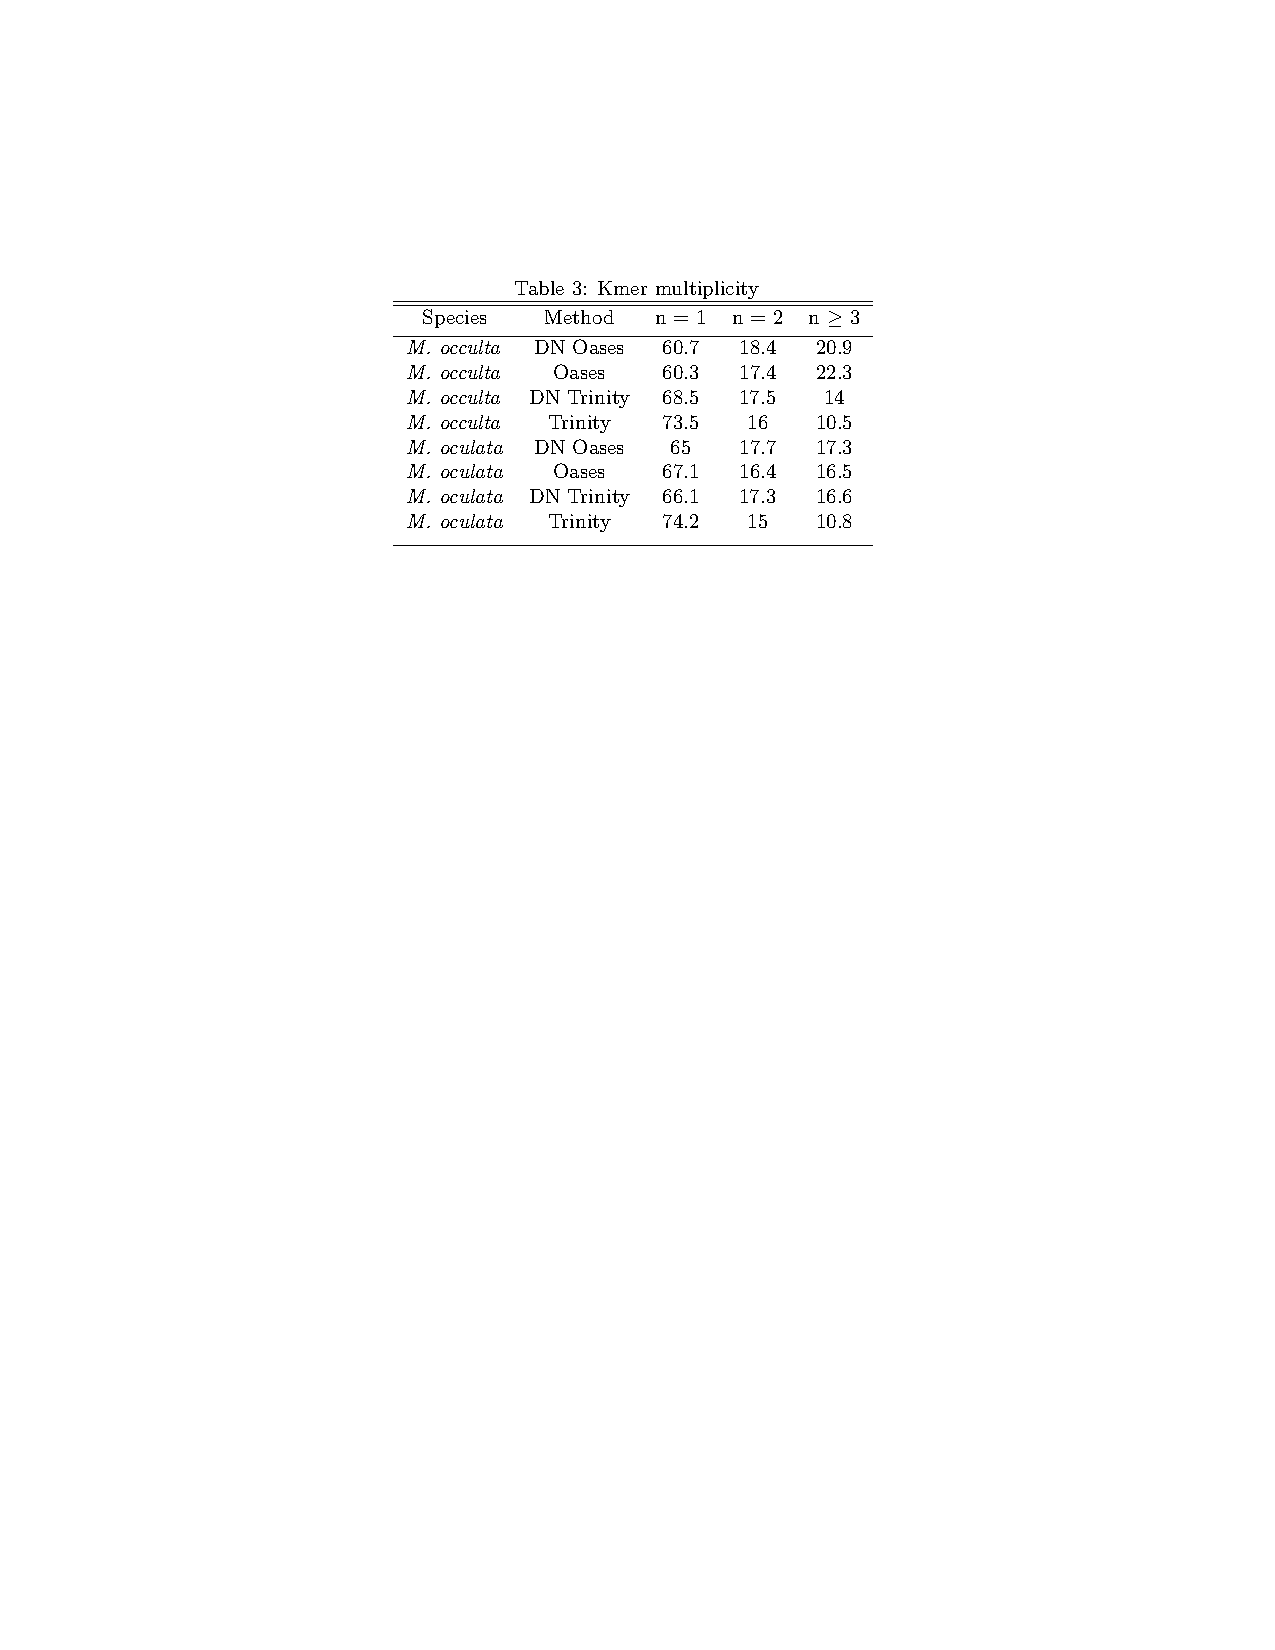
\includegraphics[width=0.4\linewidth]{Table_3_multiplicity.pdf}
\caption{\textbf{Multiplicity.} The kmer multiplicity shows uniqueness of each assembly. All kmers with a multiplicity of one are unique. Trinity has a higher percentage of unique kmer for when comparing assemblers. The unnormalized Trinity had the highest number of unique kmers overall.}
\label{fig:multiplicity}
\end{table}

\subsection{Read mapping shows high inclusion of reads in the assembled transcriptomes}
	We mapped the quality-filtered reads to the assembled transcriptomes to evaluate their inclusiveness. The F+3 stage of reads from \textit{M. occulta} had the lowest percentage of mapped reads, with the Oases unnormalized assembly mapping only 49\% of the reads, and the Trinity unnormalized assembly mapping 67\% (Figure 3\ref{fig:figure_3_mocc_mapping}). This was an isolated case: all other Oases assemblies contained at least 75\% of the reads for each time point and the Trinity assemblies contained at least 93\% of the reads for each time point. Trinity raw read assemblies tended to contain slightly more reads than the diginorm assemblies, while the opposite was true for Oases; however, in no case did the raw-reads assembly differ from the diginorm assemblies in more than 3\% of their read content.
\setcounter{subfigure}{0}
\begin{figure}[tbp]
	\begin{center}
	\subfigure[]{%
                \label{fig:figure_3_mocc_mapping}
                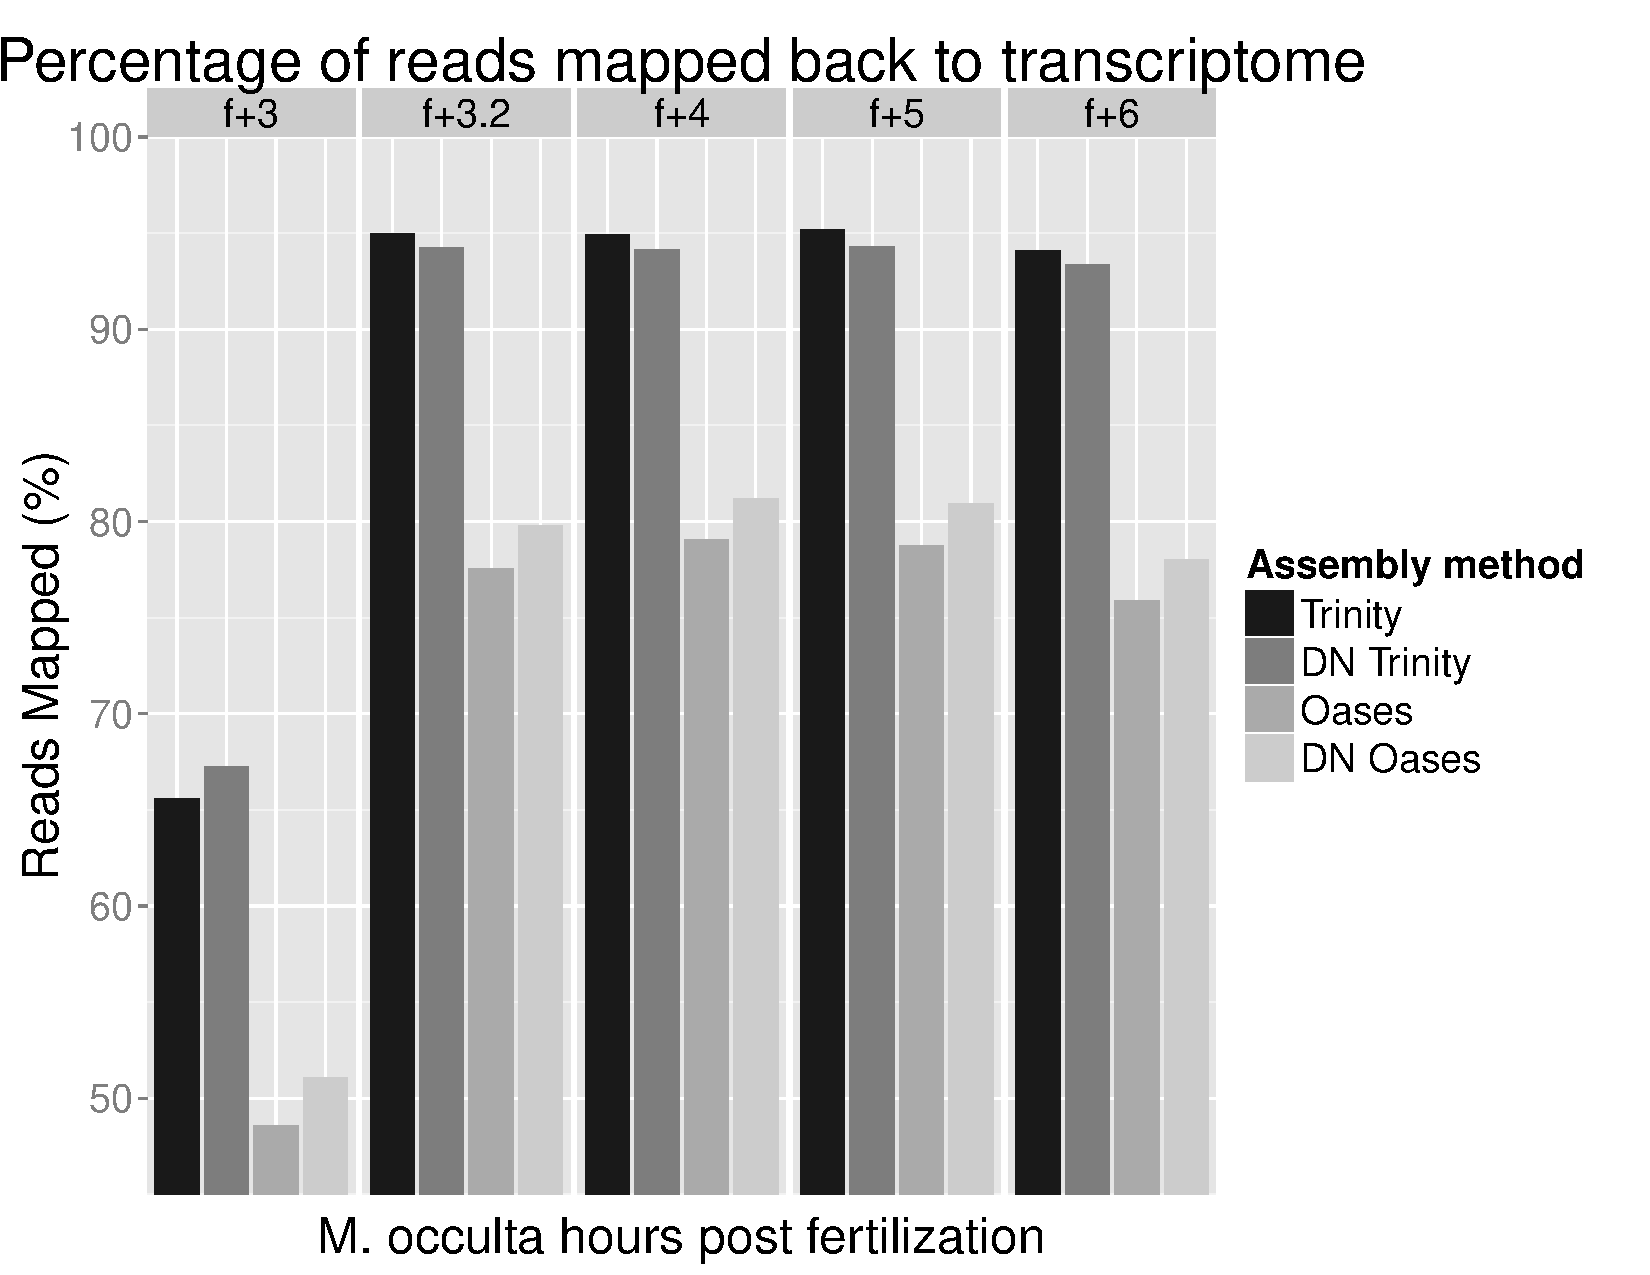
\includegraphics[width=0.4\textwidth]{figure_3_mocc_mapping.pdf}
	}%
	\subfigure[]{%
                \label{fig:figure_3_mocu_mapping}
                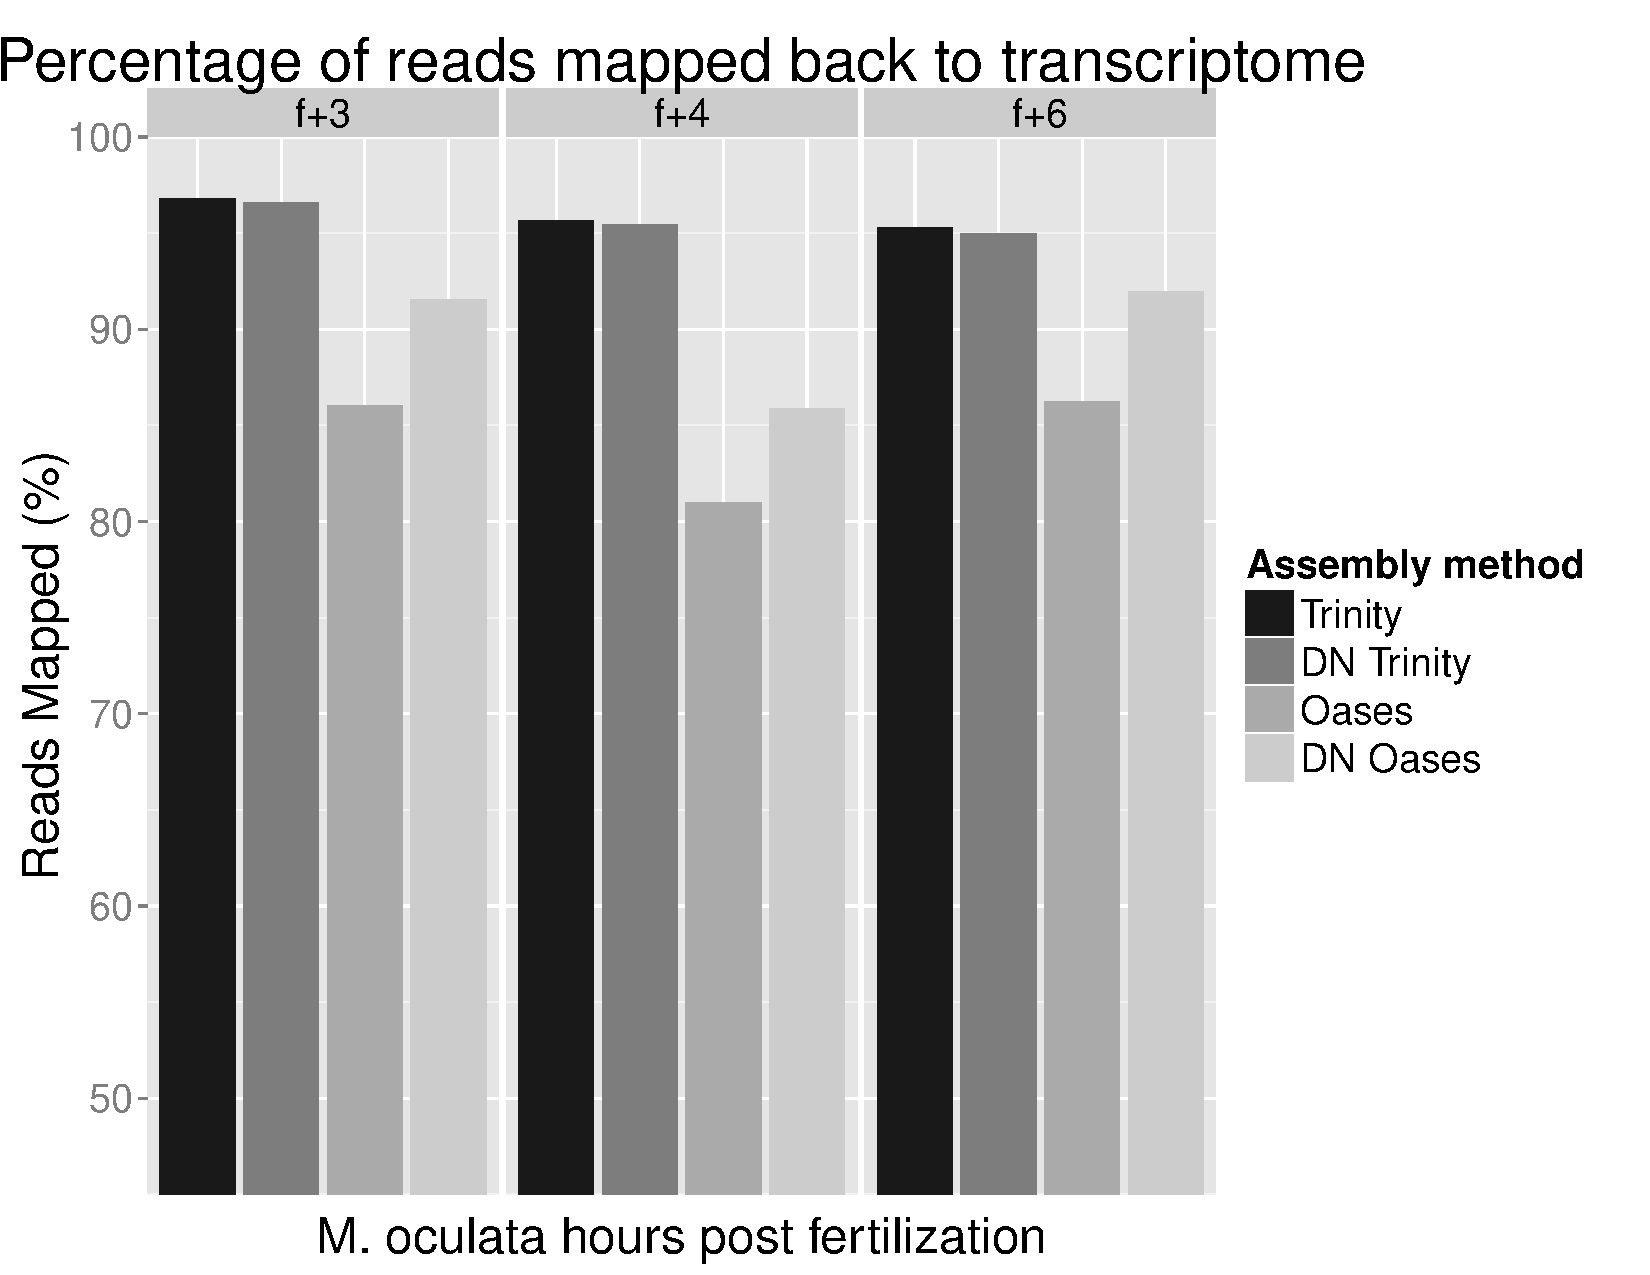
\includegraphics[width=0.4\textwidth]{figure_3_mocu_mapping.pdf}
	}%
	\end{center}
	\caption{\textbf{Read mapping.} Unnormalized reads were mapped back to each of the assemblies to determine the inclusion of reads in the assembly. ~\ref{fig:figure_3_mocc_mapping}\textit{M. occulta} first round of gastrulation reads (f+3), showed the lowest mapping quality for all assemblies, the lowest being Raw Oases at 48.57\%. \textit{M. occulta} f+3 is the only case were mapping is less than 74\% and the only case where DN Trinity mapped more reads than Raw Trinity. ~\ref{fig:figure_3_mocu_mapping}\textit{M. oculata} unnormalized Oases preformed the worse, with Trinity assemble having the best mappings.Trinity assemblies have more mapped reads than Oases for all conditions, having at least 93\% read mapping for both species. Raw Trinity typically mapped slightly more reads than DN, and the opposite occurs for Oases, with DN having more reads mapped to its assembly.}
	\label{fig:read_mapping}
\end{figure}

\subsection{All assemblies recovered transcripts with high accuracy but varied completeness}
mRNAseq assembly accuracy can be calculated based on known transcripts generated from longer reads or reference genomes \citep{vijay_challenges_2012,martin_next-generation_2011}. We use Molgulid nucleotide sequences from NCBI to measure accuracy, and we define accuracy as the average BLAST identity score for the best match for each gene recovered \citep{li_sequence_2009}. There are 178 sequences from within the Molgula clade in the NCBI database. With the exception of \textit{M. occulta} unnormalized Oases assembly, all assemblies have hits to at least 113 out of these Molgula sequences (Figure 4). The Trinity assemblies for both species have hits to all 178 sequences. Oases assemblies have hits for more sequence using digital normalized reads, two additional hits for \textit{M. oculata} and 40 additional hits for \textit{M. occulta}. \textit{M. oculata} assemblies hits have high average accuracy in the 90 and 99 percentile for Oases and Trinity, respectively. Completeness is the percentage of a gene, transcript or protein that is recovered. Within the \textit{M. oculata} assemblies, the unnormalized Oases assembly has the lowest average completeness at 36\%, the Trinity assemblies round out at 60\% and the digital normalized Oases assembly has the highest average completeness at 72\%.

\setcounter{subfigure}{0}
\begin{figure}[tbp]
	\begin{center}
	\subfigure[]{%
                \label{fig:figure_4_moccVsknownmolg}
                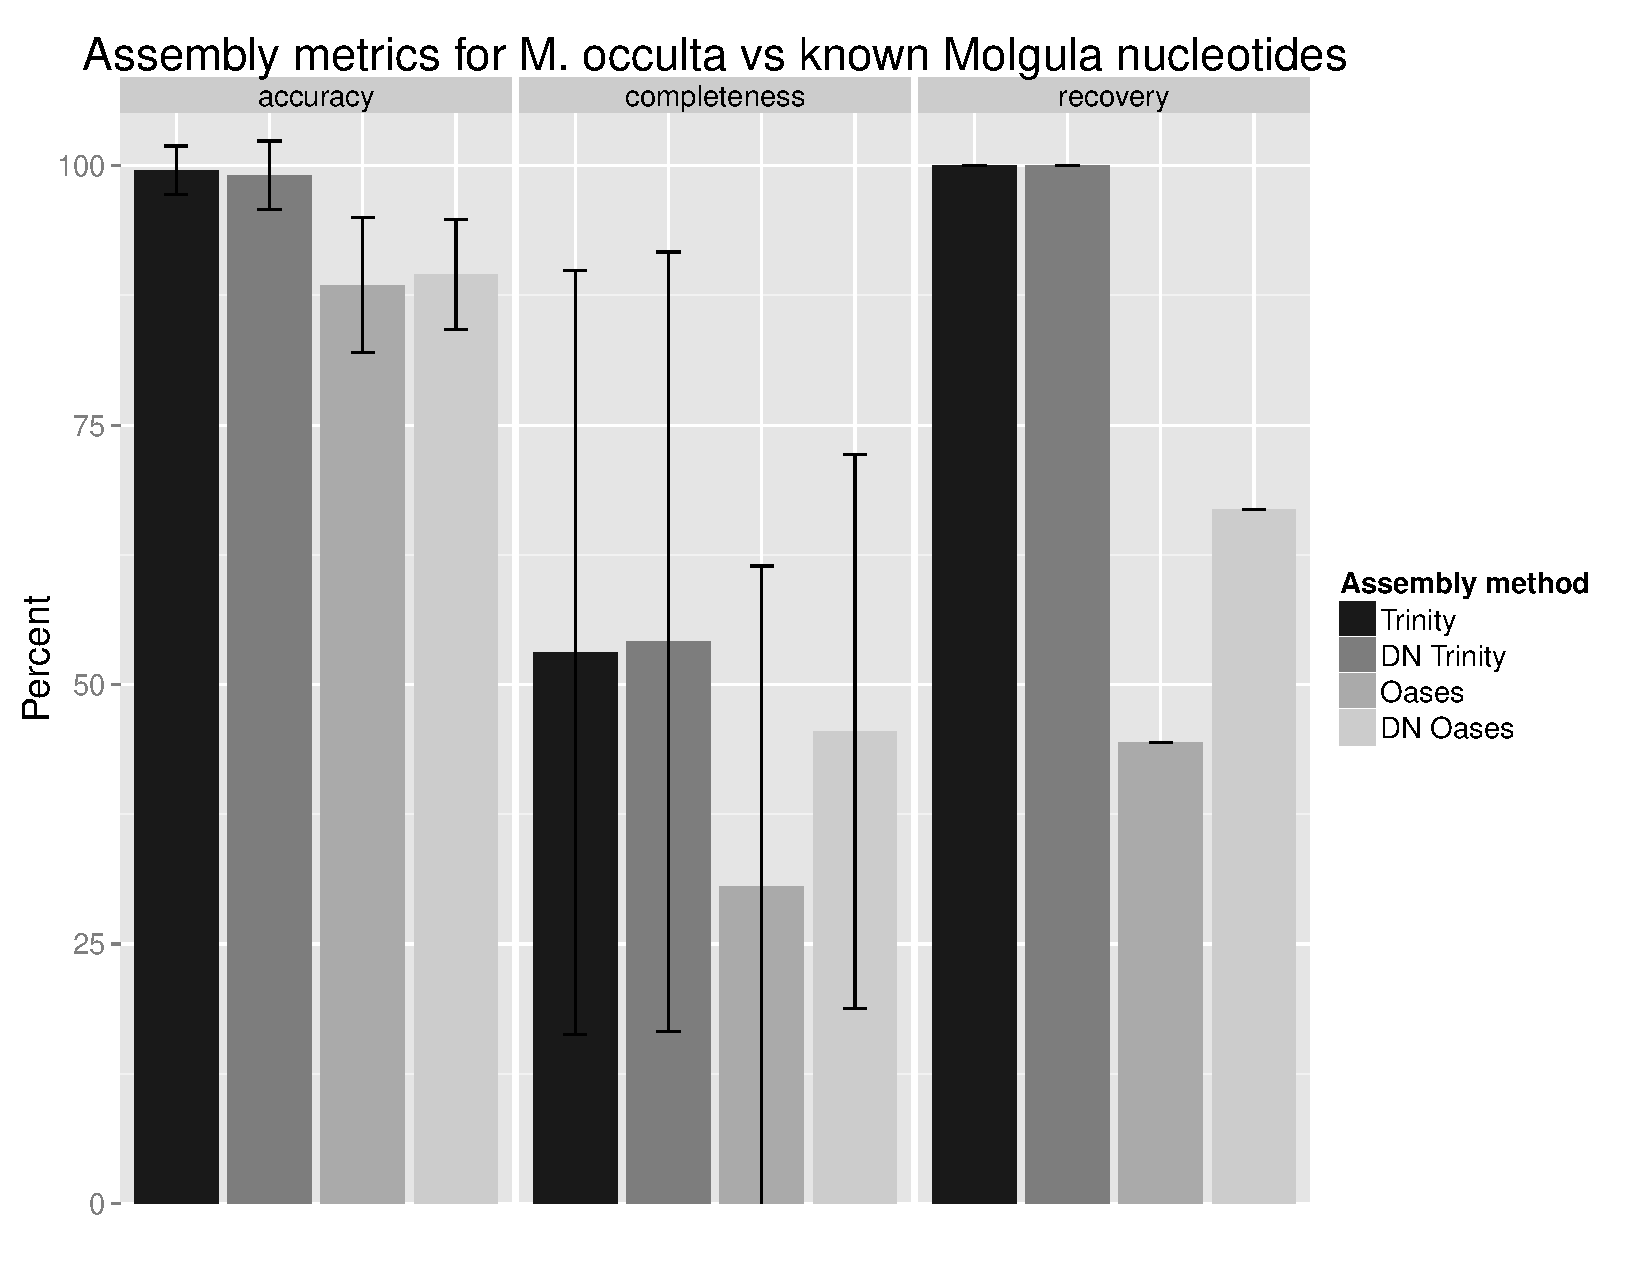
\includegraphics[width=0.4\textwidth]{figure_4_moccVsknownmolg.pdf}
	}%
	\subfigure[]{%
                \label{fig:figure_4_mocuVsknownmolg}
                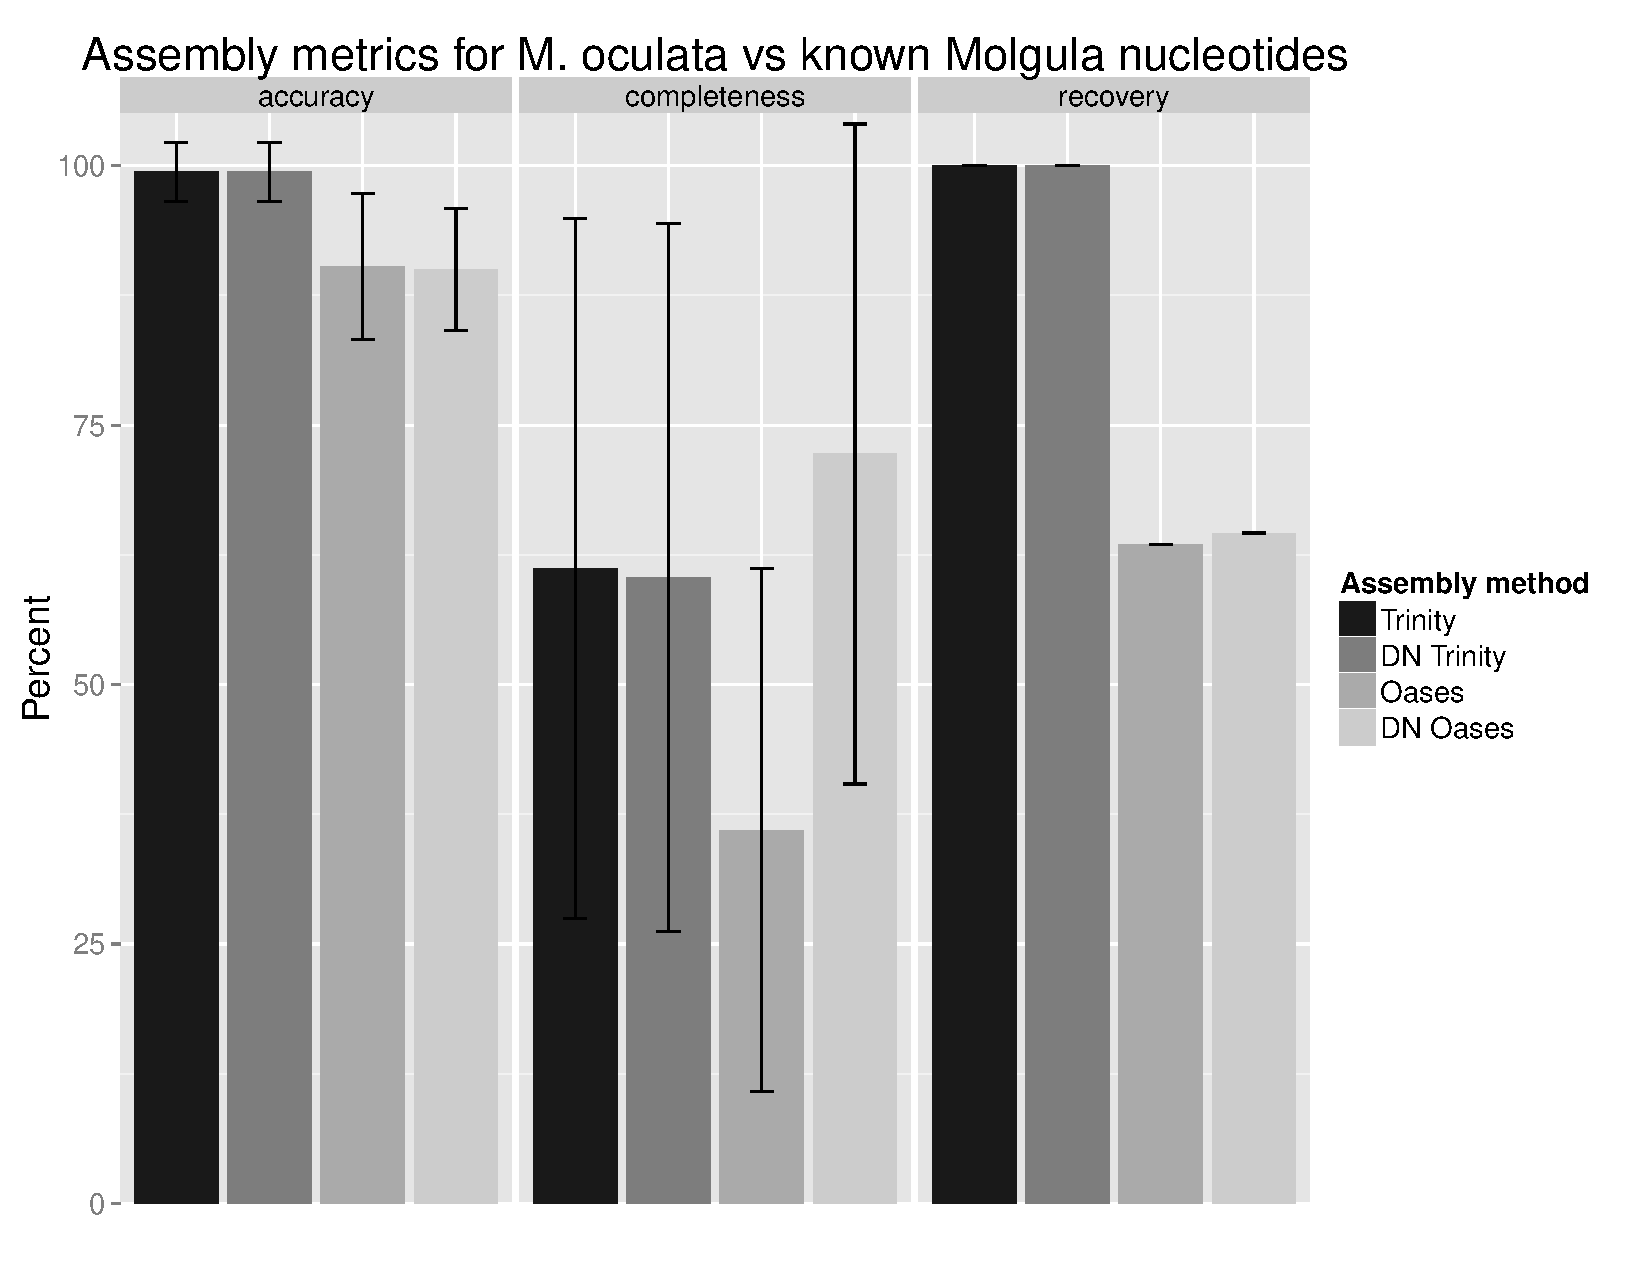
\includegraphics[width=0.4\textwidth]{figure_4_mocuVsknownmolg.pdf}
	}%
	\end{center}
	\caption{\textbf{Accuracy, completeness and recovery rate against know Molgula sequences.} The NCBI has 178 Molgula sequence in its database. Transcripts were BLAST against these sequences using BLASTN with a cut-off of e-12. Trinity assemblies preformed the best, recovering all known sequences. \textit{M. occulta} unnormalized assembled preformed the worst, only recovering 79 (44\%) of the transcripts. \textit{M. occulta} tended to recover less of the known transcripts as well.}
	\label{fig:known_molg}
\end{figure}
     
Of these 178 nucleotide sequences, 8 of them are \textit{M. occulta} sequences and 15 of them are \textit{M. oculata} sequences. All \textit{M. occulta} assemblies recovered all 8 of the NCBI \textit{M. occulta} sequences with a 94\% or greater accuracy. \textit{M. oculata} assemblies recovered \textit{M. oculata} transcripts at a 93\% accuracy as well. \textit{M. occulta} assemblies produced the lowest completeness of the two species, 41\% and 43\% for unnormalized Oases and Diginorm Oases respectively, and 75\% for both Trinity assemblies. \textit{M. oculata} assemblies produced more complete transcripts 66, 75, 86, and 83 percent for unnormalized Oases, Diginorm Oases, unormalized Trinity and Diginorm Trinity respectively.


\subsection{Both unnormalized and normalized assemblies recovered many of the same transcripts}
We next evaluated the two diginorm and unnormalized assemblies against one another to test whether either method missed significant portions of the transcriptome assembled by the other. We used BLAT to compare unnormalized and diginorm assemblies in both directions. In \textit{M. occulta}, both methods recovered at least 93\% of the transcripts, with Trinity diginorm recovering \mytilde99\% of trinity's unnormalized. \textit{M. oculata} assemblies showed high overlap as well, all recovering greater than 98\% of each other with the exception of diginorm Oases recovering 94\% of unnormalized Oases assembly.

\subsection{Homology search against the \textit{Ciona} proteome shows similar recovery of ascidian genes across assemblies}
We next used \textit{Ciona intestinalis} to evaluate the completeness of our transcriptomes. \textit{C. intestinalis} has an assembled genome that is well annotated and is the closest available genome to the Molgulids. \textit{C. intestinalis} has a genome of ~160 Mb and contains \mytilde16,000 genes \citep{satoh_surfing_2005}. A total of 13, 835 (86\%) of the \textit{C. intestinalis} proteins found in NCBI had hit in the \textit{M. occulta} transcriptomes (Figure 5), with 2,288 genes (14\%) having no hits due, presumably to either lack of expression, high divergence, or lack of presence in \textit{M. occulta}. When comparing transcripts excluded by either diginorm or unnormalized reads for all assemblies, the unormalized read assemblies produced an additional 0.04\% hits to \textit{C. intestinalis} and there was additional 0.03\% for the diginorm assemblies. There was little difference between the assemblies when compared to \textit{C. intestinalis}, with 99\% of the \textit{C. intestinalis} genes being found in all \textit{M. occulta} assemblies (Figure 4a). Eighty-six percent of the \textit{C. intestinalis} proteins had matches in the \textit{M. occult} and \textit{M. oculata} assemblies with less than 1\% difference in presence between the several assemblies (Figure 4b).
     
 \setcounter{subfigure}{0}
\begin{figure}[tbp]
	\begin{center}
	\subfigure[\textit{ M. occulta}]{%
                \label{fig:figure_5_mocc_blast_overlap}
                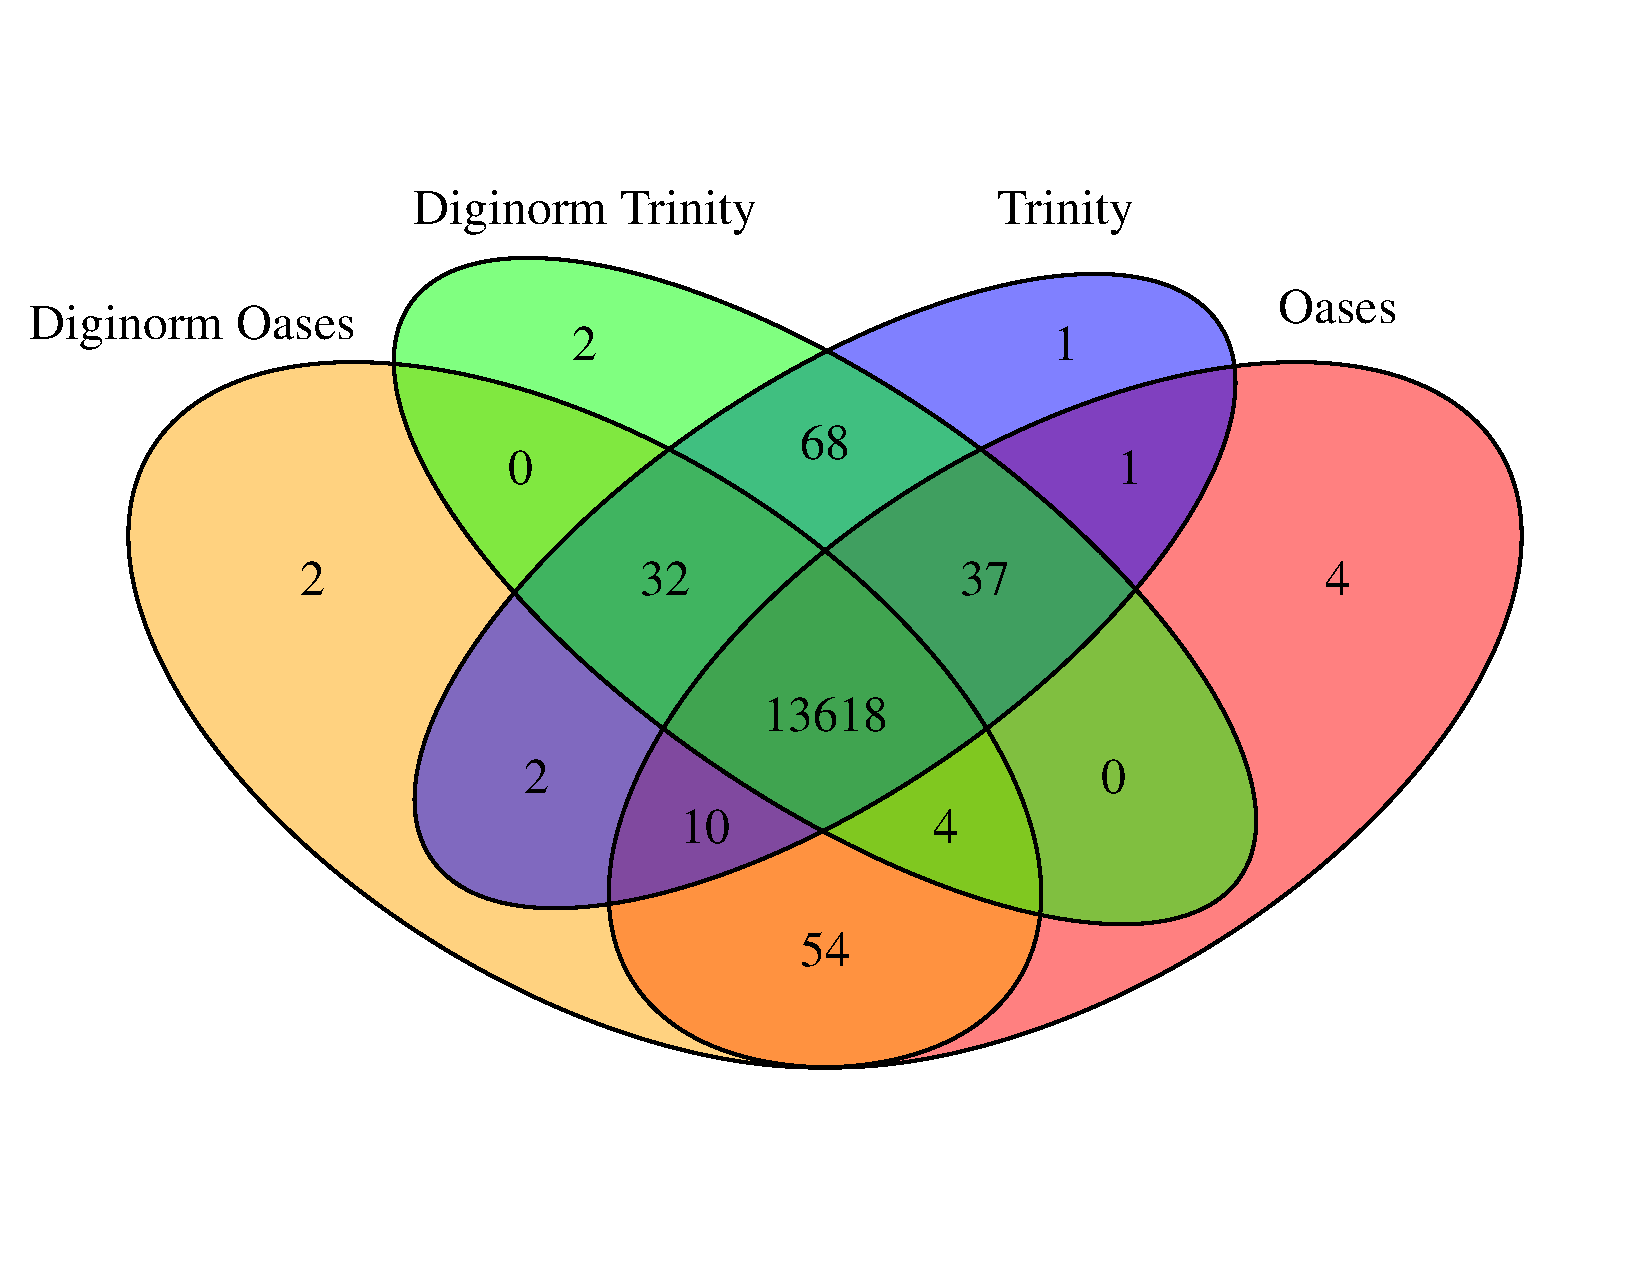
\includegraphics[width=0.4\textwidth]{figure_5_mocc_blast_overlap.pdf}
	}%
	\subfigure[\textit{ M. oculata}]{%
                \label{fig:figure_5_mocu_blast_overlap}
                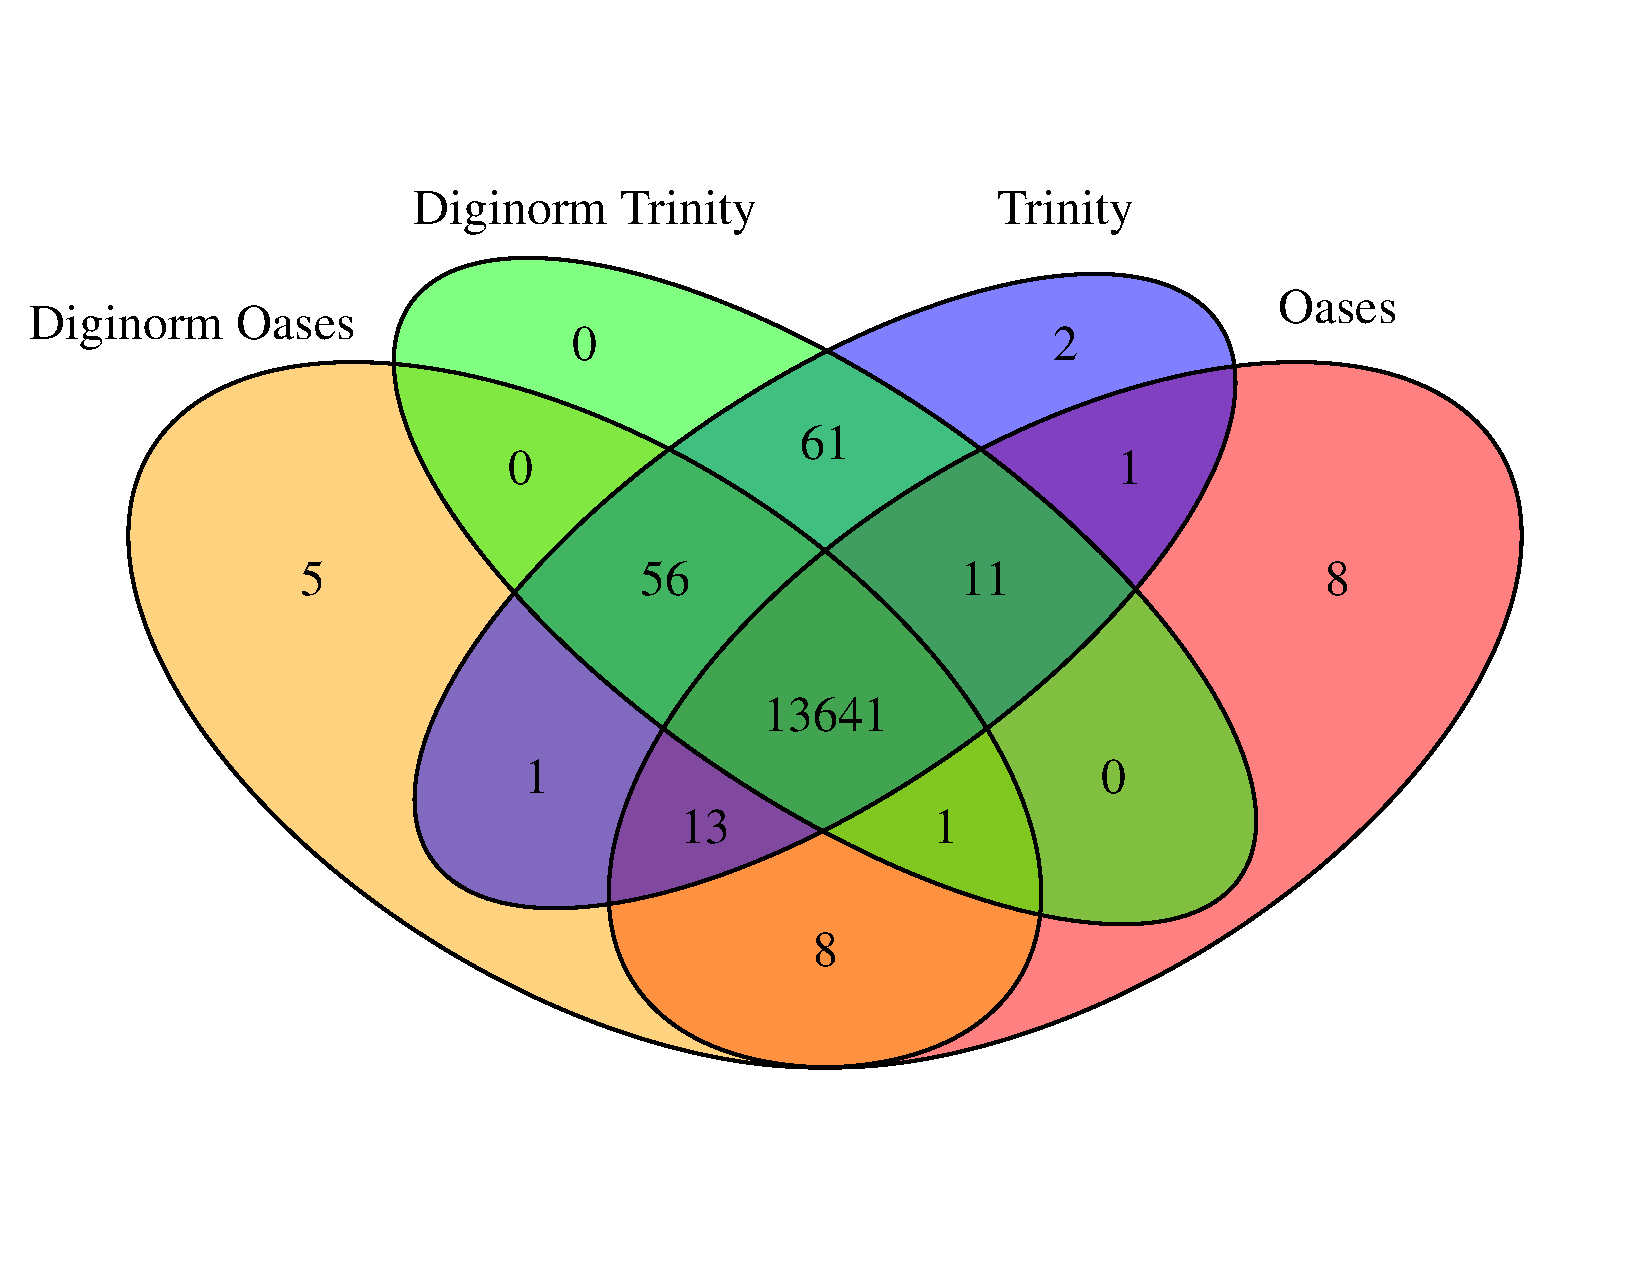
\includegraphics[width=0.4\textwidth]{figure_5_mocu_blast_overlap.pdf}
	}%
	\end{center}
	\caption{\textbf{Gene recovery, raw reads versus Normalized.} Gene homologue with C. intestinalis via BLAST for M. occulta (left) and M. oculata (right). Each oval represent the total number of homologs sequences recovered. In both species the trinity assembler assembled more homologous sequences. There was strong overlap in homology for both assemblers and both assembly conditions.}
	\label{fig:overlap}
\end{figure}
     
We next examined the difference between the unnormalized and digitally normalized assemblies. Transcripts in the unnormalized assembly with BLAST hits to \textit{C. intestinalis} but without hits in diginorm assemblies were extracted, and searched using BLASTN against the diginorm assemblies; we found fragmented versions of these transcripts, suggesting that they were partially assembled.  We then mapped the diginorm reads to the extracted unormalized transcripts and found that some portions of the transcripts were not covered by the normalized reads. This demonstrates that these transcripts were lost due to a loss of information from the diginorm process.  However, the overall loss was minimal and complemented by an increase in the recovery of other conserved transcripts; this is clearly a direction for further study.
\subsection{CEGMA analysis shows high recovery of genes}
CEGMA uses a list of highly conserved eukaryotic proteins to evaluate genome and transcriptome completeness \citep{parra_cegma:_2007}. We used CEGMA to analyze the number of protein families that are present in each assembly. The default CEGMA parameters were used for analysis. CEGMA reports recovery as ``complete'' or ``partial'', where a match is marked as ``complete'' if 70\% or more of the amino acid sequence is recovered. More than 90\% of the CEGMA genes were recovered completely in each of the transcriptome assemblies, while greater than 98\% of the CEGMA genes were recovered at least partially. 

\section{Discussion}

\subsection{Transcriptome assembly accurately recovers known transcripts and many genes}
Diginorm increased the recovery rate for the known Molgula nucleotides for the Oases assemblies. Diginorm did not have much of an effect on \textit{M. oculata}, however, \textit{M. occulta} which has 10 of millions more reads, had a much more noticeable effect, a 51\% increase in recovered sequences. Diginorm also had a positive effect on the completeness of transcripts when assembling with Oases. Trinity performed better than Oases whether the reads are digitally normalized or unnormalized. Completeness was not over 60\% for any of the assemblies, but these can be explained by the fact that most of the nucleotide sequences were not mRNA so our transcripts would not align to the intronic regions. This confirms that all assembly techniques yielded good transcriptomes when applied to both data sets.

All of the transcriptome assemblies also yielded homologs for an almost identical subset of the \textit{Ciona intestinalis} proteome.  While the evolutionary distance between the Molgulids and \textit{C. intestinalis} may be large -- the Molgulids are stolidobranch ascidians and are believed to be very divergent from \textit{C. intestinalis}, which is a phlebobranch ascidian \citep{huber_evolution_2000, stach_phylogeny_2002}\textemdash approximately 84\% of \textit{Ciona} proteins were found in all assemblies via BLAST, and more than 44\% of \textit{Ciona} proteins had putative orthologs in each of our assemblies via reciprocal best hit.  Since both transcriptomes are from a limited set of embryonic tissues that do not express all genes, these are surprisingly high numbers!  We infer that we have recovered almost all embryonic genes and the majority of genes present in the Molgula genomes.

Read mapping and CEGMA analyses further confirm that the transcriptome assemblies are of high quality and inclusiveness.  The assemblies represent 75\% or more of the reads from all but one time point, contain complete matches to 90\% or more of the conserved eukaryotic gene families in CEGMA, and contain partial matches to 98\% or more of the CEGMA families.   It is important to note that the CEGMA results are almost certainly biased upwards by the nature of the CEGMA families, which represent many more metabolic and cellular function genes than e.g. animal-specific transcription factors; thus the CEGMA numbers do not directly demonstrate the inclusiveness of the transcriptome families, as they would for a genome assembly \citep{parra_cegma:_2007}.

\subsection{Digital normalization eases assembly without strongly affecting assembly content}

One of our goals in this study was explore the biological implications of digital normalization on transcriptome assemblies; while previous studies have shown that digital normalization can make assembly faster and less memory intensive, gene recovery has been less well studied \citep{haas_novo_2013, brown_reference-free_2012, pell_scaling_2012}.  Here we confirm the computational results: diginorm dramatically reduces the computational cost of Oases assemblies, and also decreases the time and memory requirements for Trinity assemblies.

While digital normalization does alter the number of transcripts significantly, it does not strongly affect either read inclusion or the conserved gene content of the assemblies. Read inclusion by mapping never decreased more than 3\% after digital normalization, and in many cases increased. The conserved gene content, measured by a proteome comparison, showed that we recover essentially the same set of proteins with all four treatments on both transcriptomes.  

Combined, these results suggest that the varying number of transcripts largely reflect differences in the splice variants reported by different assemblers under different conditions. These results also strongly support the idea that preprocessing with digital normalization does not strongly affect assembly content.  We note, however, that the few transcripts not recovered in assemblies of the digitally normalized reads were probably not recovered because the underlying reads were eliminated during digital normalization.  This is an area where digital normalization can be improved.

Only a small number (well below 1\%) of different homology matches were reported between the various assemblies.  Because of this we decided not to merge or otherwise combine the different assemblies: the likely benefits were outweighed by the risk of introducing chimeric transcripts or combining isoforms.

We also note that the variation in number of assembled transcripts due to read preprocessing and choice of assembler despite the similar gene content suggests that traditional genome assembly metrics such as number of transcripts, total bp assembled, and N50 are not useful for transcriptome evaluation as previously suggested \citep{oneil_assessing_2013}.  For example, the same exon may be included in multiple splice variants, inflating the total bp assembled; some assemblers may choose to report more isoforms than others even with the same read support; and N50 makes little sense for transcriptomes.
 
\subsection{Trinity assemblies are more sensitive to low-abundance k-mers but contain no new conserved genes}
The difference in transcript numbers between Trinity and Oases assemblies is stark: for the same data set, with the same treatment, Trinity always produces thousands more transcripts than Oases.  Moreover, many more reads can be mapped to the Trinity assemblies \textemdash 10\% or more, for every tissue.  Despite this greater inclusion of reads, we see no substantial gain in either CEGMA matches or \textit{Ciona} proteome matches for the Trinity assemblies.

This conundrum can be resolved by examining the k-mer spectra, which show that the Trinity assemblies include many more low-abundance k-mers from the read data set.  This demonstrates that Trinity is more sensitive to low-abundance sequences, and may include more isoforms in its assemblies\textemdash by design, Trinity attempts to be more sensitive to isoforms than Oases, and focuses particularly on low-coverage isoforms \citep{vijay_challenges_2012, grabherr_full-length_2011, van_belleghem_novo_2012}. Those transcripts were indeed the results of trinity assembling low coverage reads, having an average coverage of 5x compared to 75x. To confirm this, we examined the multiplicity of k-mers in the assemblies; many more k-mers show up two or more times in the Trinity assemblies, suggesting that they are shared between multiple isoforms.
 
\section{Conclusions}
We show that transcriptome assembly on two closely related species of Molgulid ascidians produced accurate and high-quality transcriptomes, as determined by several different metrics.  Importantly, four different assembly protocols produced transcriptomes that contained nearly identical complements of homologs to the nearest model organism, \textit{Ciona intestinalis}.  While variations in isoform content were observed, these variations had little apparent impact on sensitivity of homologous gene recovery. We provide detailed assembly protocols that should enable others to easily achieve \textit{de novo} transcriptome assemblies.

\section*{Acknowledgments}

Elijah Lowe and this research were supported by the National Science Foundation under Cooperative Agreement No. DBI-0939454 (BEACON). Any opinions, findings, and conclusions or recommendations expressed in this material are those of the authors and do not necessarily reflect the views of the National Science Foundation.

\bibliography{MyLibrary}

\end{document}